\chapter{Gráficas}

\textbf{NOTA:} Siempre que se habla de un intervalo $(a,b)$, el número $a$ es menor que el $b.$\\\\

    %--------------------ejemplo
    \begin{ejem}
	Hallar la función $f$ cuya gráfica pasa por $(a,b)$ y $(c,d)$. Esto equivale a decir que $f(a)=b$ y $f(c)=d.$\\\\
	    Respuesta.-\; Si $f$ ha de ser de la forma $f(x)=\alpha x + \beta$, entonces se debe tener $$\alpha a + \beta = b,$$ $$\alpha c + \beta = d$$
	    por lo tanto, $\alpha = (d-b)/(c-a)$ y $\beta = b - \left[()d-b/c-a\right]a$, de manera que:
	    $$f(x)=\dfrac{d-b}{c-a}x + b - \dfrac{d-b}{c-a}a = \dfrac{d-b}{c-a}(x-a) +b, \qquad si \; a\neq c$$\\
     \end{ejem}

\section{Problemas}

\begin{enumerate}[\large\bfseries 1.]

    %--------------------1.
    \item Indíquse sobre una recta el conjunto de todas las $x$ que satisfacen las siguientes condiciones. Dar también un nombre a cada conjunto, utilizando la notación para los intervalos ( en algunos casos será necesario también el signo $\cup$).\\\\
    \begin{enumerate}[\bfseries (i)]
	
	%----------(i)
	\item $|x-3| < 1$\\\\
	    Respuesta.-\; $-1< x-3 <1 \quad \Longrightarrow \quad 2 < x < 4$\\

	%----------(ii)
	\item $|x-3|\leq 1$\\\\
	    Respuesta.-\; $2 \leq x \leq 4$\\

	%----------(iii)
	\item $|x-a| < \epsilon$\\\\
	    Respuesta.-\; $a-\epsilon < x < a+e$\\\\
	
	%----------(iv)
	\item $|x^2 - 1| < \dfrac{1}{2}$\\\\
	    Respuesta.-\; $\pm\sqrt{\dfrac{1}{2}} < x < \pm \sqrt{\dfrac{3}{2}}$\\\\

	%----------(v)
	\item $\dfrac{1}{1+x^2} \geq \dfrac{1}{5}$\\\\
	    Respuesta.-\; $x^2-4\geq 0 \quad \Longrightarrow \quad x\geq 2 \lor x\leq -2$\\\\

	%----------(vi)
	\item $\dfrac{1}{1+x^2} \leq a$\\\\
	    Respuesta.-\; $|x| \geq \pm \sqrt{\frac{1}{a}-1}$\\\\

	%----------(vii)
	\item $x^2+1 \geq 2$\\\\
	    Respuesta.-\; $x\geq \pm 1$\\\\

	%----------(viii)
	\item $(x+1)(x-1)(x-2)>0$\\\\
	    Respuesta.-\; $x+1\geq 0 > \land x-1 > 0  \land x-2>0 \quad \Longrightarrow \quad -1<x<1 \cup x>2$\\\\

    \end{enumerate}

    %--------------------2.
    \item Existe un procedimiento muy útil para descubrir los puntos del intervalo cerrado $[a,b]$ (Suponiendo como siempre que es $a<b$)
    \begin{enumerate}[\bfseries (a)]
	
	%----------(a).
	\item Consideremos en primer lugar el intervalo $[0,b]$, para $b>0$. Demostrar que si $x$ está en $[0,b]$,entonces $x=tb$ para cierto $t$ con $0\leq t \leq 1$ ¿Cómo se puede interpretar el número $t$? ¿Cuál es el punto medio del intervalo $[0,b]$?\\\\
	    Demostración.-\; Sea $0\leq x \leq b$ entonces $0\leq \dfrac{x}{b} \leq 1$, luego sabemos que $0\leq t \leq 1$ por lo tanto $x=\dfrac{x}{b}\cdot b$. Ya que $t=\dfrac{x}{b}$, $t$ representa la razón en la que $x$ divide el intervalo $[0,b]$. Por último el punto medio del intervalo viene dado por $b/2$.\\\\

	%----------(b).
	\item Demostrar ahora que si $x$ está en $[a,b]$, entonces $x=(1-t)a+tb$ para un cierto $t$ con $0\leq t \leq 1.$ Ayuda: esta expresión se puede poner también en la forma $a+t(b-a).$ ¿Cuál es el punto medio del intervalo $[a,b]$? ¿Cuál es el punto que está a $1/3$ de camino de $a$ a $b$?\\\\
	    Demostración.-\; Sea $a\leq x \leq b$ entonces $0\leq x-a \leq b-a$, por la parte $(a)$ se tiene  $x-a=t(b-a)$ de donde $x=a+t(b-a)$\\
	    Luego el punto media del intervalor viene dado por $a+\dfrac{b-a}{2}=\dfrac{a+b}{2}$ y la tercera parte viene dado por $a+\dfrac{b-a}{2}=\dfrac{2}{3}a + \dfrac{1}{3}b.$\\\\

	%----------(c)
	\item Demostrar a la inversa que si $0\leq t \leq 1$, entonces $x=(1-t)a+tb$ esta en $[a,b]$\\\\
	    Demostración.-\; Sea $0\leq t \leq 1$ entonces $a\leq bt\leq b$ y $0\leq at\leq a$ entonces $0\leq bt-at\leq b-a$ de donde $a\leq bt-at+a \leq b$ así queda demostrado que $a\leq (1-t)a + tb \leq b$.\\\\

	%----------(d)
	\item Los puntos del intervalo abierto $(a,b)$, entonces $x=(1-t)a + tb$ para $0<t<1.$\\\\
	    Demostración.-\; la demostración es similar al inciso $(b)$.\\\\

    \end{enumerate}
    
    %--------------------3.
    \item Dibujar el conjunto de todos los puntos $(x,y)$ que satisface las siguientes condiciones. (En la mayor parte de los casos la imagen será una parte apreciable del plano y no simplemente una recta o una curva.)\\\\

    %--------------------4.
    \item Dibujar el conjunto de los puntos $(x,y)$ que satisfacen las siguientes condiciones:\\\\

    %--------------------5.
    \item Dibujar el conjunto de los puntos $(x,y)$ que satisfacen las siguientes condiciones:\\\\

    %--------------------6.
    \item 
    \begin{enumerate}[\bfseries (a)]
	
	%----------(a)
	\item Demostrar que la recta que pasa por $(a,b)$ y de pendiente $m$ es la gráfica de la función $f(x)=m(x-a)+b.$ Esta fórmula, conocida como forma punto-pendiente, es mucho más conveniente que la expresión equivalente $f(x)=mx+(b-ma)$; con la formula punto-pendiente queda inmediatamente claro que la pendiente es $m$ y que el valor de $f$ en $a$ es $b$.\\\\
	    Demostración.-\; Obsérvese simplemente que la gráfica de $f(x)=m(x-a)+b=mx+(b-ma)$ es una recta de pendiente $m$, que pasa por el punto $(a,b)$.\\\\

	%----------(b)
	\item Para $a\neq c$, demostrar que la recta que pasa por $(a,b)$ y $(c,d)$ es la gráfica de la función $$f(x)=\dfrac{d-b}{c-a}(x-a)+b$$
	    Demostración.-\; Se sabe que la pendiente esta dado por $\dfrac{d-b}{c-a}$  ya que $a\neq c$ y por la parte $(a)$ queda demostrado la proposición.\\\\
	
	%----------(c)
	\item ¿Cuáles son las condiciones para que las gráficas de $f(x)=mx+b$ y $g(x)=m^{'} x + b^{'}$ sean rectas paralelas?\\\\
	    Respuesta.-\; Cuando $m=m^{'}$ y $b\neq b^{'}$.\\\\

    \end{enumerate}

    %--------------------7.
    \item 
    \begin{enumerate}[\bfseries (a)]

	%----------(a)
	\item Si $A$, $B$ y $C$, siendo $A$ y $B$ distintos de $0$, son números cualesquiera, demostrar que el conjunto de todos los $(x,y)$ que satisfacen $Ax+By+C=0$ es una recta (que puede ser vertical). Indicación: Aclarar primero cuándo se tiene una recta vertical.\\\\
	    Demostración.-\; Si $B=0$ y $A\neq 0$, entonces el conjunto es la recta vertical formada por todos los puntos $(x,y)$ con $x=-\dfrac{C}{A}$. Si $B\neq 0$, el conjunto es la gráfica de $f(x)=(-A/B)x + (-C/B)$.\\\\ 

	%----------(b)
	\item Demostrar la inversa que toda recta, incluyendo las verticales, puede ser descrita como el conjunto de todos los $(x,y)$ que satisfacen $Ax + By + C =0$.\\\\
	    Demostración.-\; Los puntos $(x,y)$ de la vertical con $x=a$ son precisamente los que satisfacen $I\cdot x + 0\cdot y + (-a) = 0$. Los puntos $(x,y)$ de la gráfica de $f(x)=mx+b$ son precisamente los que satisfacen $(-m)x + 1\cdot y + (-b)=0$.\\\\
    \end{enumerate}

    %--------------------8.
    \item 
    \begin{enumerate}[\bfseries (a)]

	%----------(a)
	\item Demostrar que las gráficas de las funciones $$f(x)=mx+b$$ $$g(x)=nx+c,$$ son perpendiculares si $mn=-1$, calculando los cuadrados de las longitudes de los lados del triángulo de la figura 29. (¿Por qué no se restringe la generalidad al considerar este caso especial en que las rectas se cortan en el origen?).\\\\
	    Demostración.-\; Sea $\sqrt{(1-1)^2+(n-m)^2} = \sqrt{(0-1)^2+(0-m)^2} + \sqrt{(1-0)^2+(n-0)^2}$ entonces $-2mn=2 \quad \Rightarrow \quad mn=-1$. Esto demuestra el resultado cuando $b=c=0$. El caso general se deduce de este caso particualar, ya que la perpendicular depende sólo de la pendiente.\\\\

	%----------(b)
	\item Demostrar que las dos rectas que consisten en todos los puntos $(x,y)$ que satisfacen las condiciones $$Ax +By +C=0$$ $$A^{'}x + B^{'} y + C^{'} = 0,$$ son perpendiculares si y sólo si $AA^{'} + BB^{'} = 0$.\\\\
	    Demostración.-\; Si $B\neq 0$ y $B^{'} \neq 0,$ estas rectas son las gráficas de $$f(x)=(-A/B)x - C/B$$ $$f(x)=(-A^{'}/B^{'})x - C/B$$ de modo que, según la parte $(a)$, las rectas son perpendiculares si y sólo si $$\left(\dfrac{A}{B}\right)\cdot \left(\dfrac{A^{'}}{B^{'}}\right)=-1$$ por lo tanto $AA^{'}+BB^{'}=0$. Si $B=0$ y $A\neq 0$, entonces la primera recta es vertical, de modo que la segunda le es perpendicular si y sólo si $A^{'}=0,$ lo cual ocurre exactamente cuando $AA^{'} + BB^{´}=0$ Análogamente para el caso $B^{'}$.\\\\

    \end{enumerate}
    
    %--------------------9.
    \item  
    \begin{enumerate}[\bfseries (a)]

	%----------(a)
	\item Utilizando el problema $1-19$ demostrar que $$\sqrt{(x_1+y_1)^2 + (x_2+y_2)^2} \leq \sqrt{x_1^2 + x_2^2} + \sqrt{y_1^2 + y_2^2}$$\\\\
	    Demostración.-\; Esta desigualdad tiene lugar si y sólo si se cumple la que se obtiene al elevar al cuadrado ambos miembros, $$(x_1+y_1)^2+(x_2+y_2)^2\leq (x_1^2+x_2^2)+(y_1^2+y_2^2)+2\sqrt{x_1^2+x_2^2}\sqrt{y_1^2+y_2^2}$$ lo cual, como puede observarse, es equivalente a la desigualdad de Schwartz.\\\\

	%----------(b)
	\item Demostrar que $$\sqrt{(x_3-x_1)^2 + (y_3-y_1)^2} \leq \sqrt{(x_2 - x_1)^2 + (y_2 - y_1)^2} + \sqrt{(x_3 - x_2)^2 + (y_3 - y_2)^2}$$
	Interpretar esta desigualdad geométrica (llamada desigualdad triangular) ¿En qué casos se satisface la igualdad?\\\\
	    Demostración.-\; Sustituyendo $x_1 = x_2-x_1, \qquad x_2=y_2-y_1, \qquad y1=x_3-x_2, \qquad y_2=y_3-y_2$  en $(a)$ queda la ecuación esperada. Esta ecuación nos dice que la longitud de un lado de un triángulo es menor que la suma de las longitudes de los otros dos.\\\\

    \end{enumerate}

    %--------------------10.
    \item Esbozar las gráficas de las siguientes funciones, trazando un número de puntos suficiente para obtener una buena idea del aspecto general. (Una parte del problema consiste en hacer una estimación acerca de cuántos puntos serían suficientes; las preguntas que se plantean tienen por objeto hacer ver que vale más discurrir un poco que trazar centenares de puntos.)
    \begin{enumerate}[\bfseries (i)]
	
	%----------(i)
	\item $f(x)=x + \dfrac{1}{x}$ (¿Que ocurre cuando $x$ está próximo a $0$ y cuando $x$ es grande? ¿Qué posición ocupa la gráfica en relación con la gráfica de la función identidad? ¿Por qué es suficiente considerar primero sólo $x$ positivos?)\\
	\begin{center}
	    \begin{tikzpicture}[scale=1,draw opacity = 0.6]
		% abscisa y ordenada
		\tkzInit[xmax= 3,xmin=-3,ymax=3,ymin=-3.5]
		\tiny\tkzLabelXY[opacity=0.6,step=1, orig=false]
		% etiqueta x, f(x)
		\tkzDrawX[opacity=0.6,label=x,right=0.3]
		\tkzDrawY[opacity=0.6,label=f(x),below = -0.6]
		%dominio y función
		\draw [domain=0.3:3,thick,gray] plot(\x,{\x + 1/\x});
		\draw [domain=-0.3:-3,thick,gray] plot(\x,{\x + 1/\x});
	    \end{tikzpicture}
	\end{center}
	\vspace{.5cm}
	    Respuesta.-\; Cuando $x$ es próximo a $0$ la función tiende al infinito, contrariamente a $x$ grande que tiende a $1$. Con respecto a la gráfica de la función identidad ocupa una similitud interesante. Es suficiente considerar solo los $x$ positivos ya que se asimila los $x$ negativos como una imagen de función impar.\\\\
	
	%----------(ii)
	\item $f(x)=x - \dfrac{1}{x}$\\
	\begin{center}
	    \begin{tikzpicture}[scale=1,draw opacity = 0.6]
		% abscisa y ordenada
		\tkzInit[xmax= 3,xmin=-3,ymax=3,ymin=-3.5]
		\tiny\tkzLabelXY[opacity=0.6,step=1, orig=false]
		% etiqueta x, f(x)
		\tkzDrawX[opacity=0.6,label=x,right=0.3]
		\tkzDrawY[opacity=0.6,label=f(x),below = -0.6]
		%dominio y función
		\draw [domain=0.3:3,thick,gray] plot(\x,{\x - 1/\x});
		\draw [domain=-0.3:-3,thick,gray] plot(\x,{\x - 1/\x});
	    \end{tikzpicture}
	\end{center}
	\vspace{.5cm}

	%----------(iii)
	\item $f(x)=x^2 + \dfrac{1}{x^2}$\\
	\begin{center}
	    \begin{tikzpicture}[scale=1,draw opacity = 0.6]
		% abscisa y ordenada
		\tkzInit[xmax= 3,xmin=-3,ymax=6,ymin=-6.5]
		\tiny\tkzLabelXY[opacity=0.6,step=1, orig=false]
		% etiqueta x, f(x)
		\tkzDrawX[opacity=0.6,label=x,right=0.3]
		\tkzDrawY[opacity=0.6,label=f(x),below = -0.6]
		%dominio y función
		\draw [domain=0.5:2.5,thick,gray] plot(\x,{\x^2 + 1/\x^2});
		\draw [domain=-0.5:-2.5,thick,gray] plot(\x,{\x^2 + 1/\x^2});
	    \end{tikzpicture}
	\end{center}
	\vspace{.5cm}

	%----------(iv)
	\item $f(x) = x^2 - \dfrac{1}{x^2}$\\
	\begin{center}
	    \begin{tikzpicture}[scale=1,draw opacity = 0.6]
		% abscisa y ordenada
		\tkzInit[xmax= 3,xmin=-3,ymax=4,ymin=-4.5]
		\tiny\tkzLabelXY[opacity=0.6,step=1, orig=false]
		% etiqueta x, f(x)
		\tkzDrawX[opacity=0.6,label=x,right=0.3]
		\tkzDrawY[opacity=0.6,label=f(x),below = -0.6]
		%dominio y función
		\draw [domain=0.5:2,thick,gray] plot(\x,{\x^2 - 1/\x^2});
		\draw [domain=-0.5:-2,thick,gray] plot(\x,{\x^2 - 1/\x^2});
	    \end{tikzpicture}
	\end{center}
	\vspace{.5cm}

    \end{enumerate}

    %--------------------11.
    \item Describir los rasgos generales de la gráfica de $f$ si
    \begin{enumerate}[\bfseries (i)]

	%----------(i)
	\item $f$ es par.\\\\
	    Respuesta.-\; La gráfica es simétrica respecto al eje vertical.\\\\

	%----------(ii)
	\item $f$ es impar.\\\\
	    Respuesta.-\; La gráfica es simétrica respecto al origen.\\\\

	%----------(iii)
	\item $f$ es no negativa.\\\\
	    Respuesta.-\; La gráfica queda sobre el eje horizontal.\\\\

	%----------(iv)
	\item $f(x)=f(x+a)$ para todo $x$ (las funciones que tienen eta propiedad reciben el nombre de periódicas con periodo $a$).\\\\
	    Respuesta.-\; La gráfica de $f$ repite una y otra vez la parte comprendida entre $0$ y $a$.\\\\

    \end{enumerate}

    %--------------------12.
    \item Trazar las funciones $f(x)=\sqrt[m]{x}$ para $m=1,2,3,4.$ (Hay una manera fácil de hacer esto, utilizando la figura 14. Recuérdese, sin embargo, que $\sqrt[m]{x}$ significa la raíz m-ésima positiva de $x$ cuando $m$ es par; se debe también tener presente que existirá una diferencia notable entre las gráficas cuando $m$ es par y cuando $m$ es impar.)\\\\
	Respuesta.-\; 
	\begin{center}
	    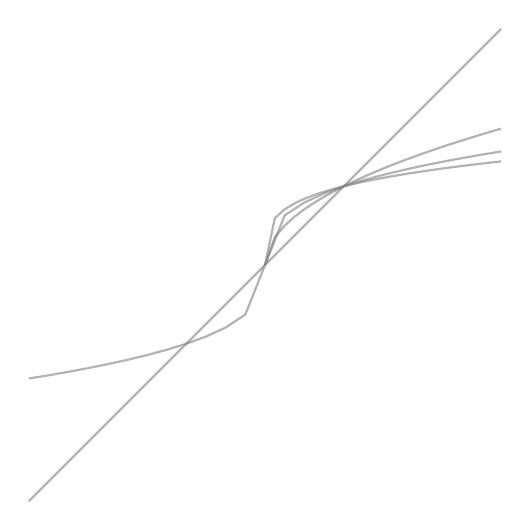
\begin{tikzpicture}[scale=1,draw opacity = 0.6]
		% abscisa y ordenada
		\tkzInit[xmax= 3,xmin=-3,ymax=3,ymin=-3]
		\tiny\tkzLabelXY[opacity=0.6,step=1, orig=false]
		% etiqueta x, f(x)
		\tkzDrawX[opacity=0.6,label=x,right=0.3]
		\tkzDrawY[opacity=0.6,label=f(x),below = -0.6]
		%dominio y función
		\draw [domain=-3:3,thick,gray] plot(\x,{\x});
		\draw [domain=0:3,thick,gray] plot(\x,{\x^(1/2)});
		\draw [domain=-3:3,thick,gray] plot(\x,{\x^(1/3)});
		\draw [domain=0:3,thick,gray] plot(\x,{\x^(1/4)});
	    \end{tikzpicture}
	\end{center}
	\vspace{.5cm}

    %--------------------13.
    \item
    \begin{enumerate}[\bfseries (a)]
	
	%----------(a)
	\item Trazar $f(x)=|x|$ y $f(x)=x^2$\\\\
	    Respuesta.-\;
	    \begin{center}
		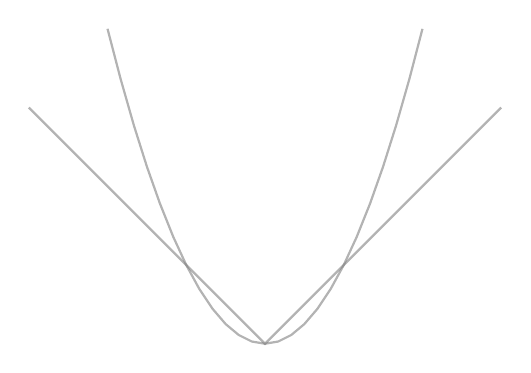
\begin{tikzpicture}[scale=1,draw opacity = 0.6]
		    % abscisa y ordenada
		    \tkzInit[xmax= 3,xmin=-3,ymax=3,ymin=-1]
		    \tiny\tkzLabelXY[opacity=0.6,step=1, orig=false]
		    % etiqueta x, f(x)
		    \tkzDrawX[opacity=0.6,label=x,right=0.3]
		    \tkzDrawY[opacity=0.6,label=f(x),below = -0.6]
		    %dominio y función
		    \draw [domain=-3:3,thick,gray] plot(\x,{abs(\x)});
		    \draw [domain=-2:2,thick,gray] plot(\x,{\x*\x});
		\end{tikzpicture}
	    \end{center}
	    \vspace{.5cm}

	%----------(b)
	\item Trazr $f(x)=|\sin x|$ y $f(x)=\sin^2 x$(Existe una diferencia importante entre las gráficas, diferencia que todavía no podemos ni siquiera describir con rigor. Inténtese descubrir en qué consiste; la parte $(a)$ está destinada a servir de orientación).\\\\
	    Respuesta.-\; La gráfica oscila como corresponde similar a $(a)$ con respecto a la analogía.\\\\ 

    \end{enumerate}

    %--------------------14.
    \item Describir la gráfica de $g$ en función de la gráfica de $f$ si:
    \begin{enumerate}[\bfseries (i)]

	%----------(i)
	\item $g(x)=f(x)+c.$\\\\
	    Respuesta.-\; La gráfica de $g$ es la gráfica de $f$ trasladada hacia arriba en $c$ unidades.\\\\

	%----------(ii)
	\item $g(x)=f(x+c)$.\\\\
	    Respuesta.-\; La gráfica de $g$ es la gráfica de $f$ trasladada $c$ unidades hacia la izquierda si $c>0$.\\\\

	%----------(iii)
	\item $g(x)=cf(x)$\\\\
	    Respuesta.-\; La altura de la gráfica de $f$ es multiplicada invariablemente por el factor $c$. Si $c=0$ esto significa que $g=0$; si $c>0$, las distancias al eje horizontal son afectadas por el factor, pero conservan el mismo sentido,; si $c<0$ se invierten los sentidos.\\\\

	%----------(iv)
	\item $g(x)=f(cx)$\\\\
	    Respuesta.-\; La gráfica de $f$ resulta contraida mediante el factor $c$ si $c>0$; si $c<0$, la contracción se combina con una simetría respecto al eje vertical. Si $c=0$, entonces $g$ es una función constante, $g(x)=f(0)$.\\\\

	%----------(v)
	\item $g(x)=f(1/x)$\\\\
	    Respuesta.-\; Todo lo que ocurre lejos de $0$, ocurre también cerca, y viceversa, lo cual queda amploamente ilustrado con gráfica de $g(x)=\sin (1/x)$.\\\\

	%----------(vi)
	\item $g(x)=f(|x|)$\\\\
	    Respuesta.-\; La gráfica de $g$ consiste en la parte de la gráfica a la derecha del eje vertical, junto con la simetría de dicha parte respecto al mismo eje vertical.\\\\

	%----------(vii)
	\item $g(x)=|f(x)|$\\\\
	    Respuesta.-\; La gráfica de $g$ se obtiene levantando hacia arriba todas aquellas partes de la gráfica de $f$ que quedan por debajo del eje horizontal.\\\\

	%----------(viii)
	\item $g(x)=max(f,0)$\\\\
	    Respuesta.-\; La gráfica de $g$ se obtiene recortando aquellas partes de la gráfica de $f$ que se encuentran por debajo del eje horizontal.\\\\ 

	%----------(ix)
	\item $g(x)=min(f,0)$\\\\
	    Respuesta.-\; La gráfica de $g$ se obtiene recortando las partes de la gráfica de $f$ que quedan por encima del eje horizontal.\\\\

	%----------(x)
	\item $g(x)=max(f,1)$\\\\
	    Respuesta.-\; La gráfica de $g$ se obtiene recortando la parte de la gráfica de $f$ que queda por debajo de la horizontal de altura $1$ sobre el eje.\\\\

    \end{enumerate}

    %--------------------15.
    \item Trazar la gráfica de $(x)=ax^2+bx+c$. Indicación: utilizar los métodos del problema $1-18$.\\\\
	Respuesta.-\; Al ser $$f(x)=ax^2+bx+c=a\left( x^2 + \dfrac{b}{a}x + \dfrac{c}{a} \right) = a \left[ \left( x + \dfrac{b}{2a} \right)^2 + \left( \dfrac{c}{a} - \dfrac{b^2}{4a} \right)  \right]$$ 
	\begin{center}
	    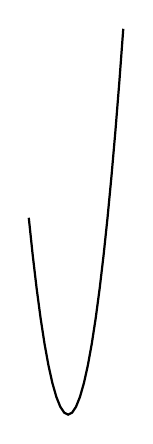
\begin{tikzpicture}
		% abscisa y ordenada
		\tkzInit[xmax=2,xmin=-2,ymax=4,ymin=0]
		\tiny\tkzLabelXY[opacity=0.6,step=1, orig=false]
		% label x, f(x)
		\tkzDrawX[opacity= .6,label=C,right=0.3]
		\tkzDrawY[opacity= .6,label=F,below = -0.6]
		%dominio y función
		\draw[domain=-3:3,thick, scale=.2] plot(\x,{2*\x*\x + 2*\x + 2}); 
	    \end{tikzpicture}
	\end{center}
	\vspace{0.5cm}

    %--------------------16.
    \item Supóngase que $A$ y $C$ no son cero a la vez. Demostrar que el conjunto de todos los $(x,y)$ que satisfacen $$Ax^2 + Bx + Cy^2 +Dy + E = 0$$ es o bien una parábola, una elipse o una hipérbola (o posiblemente $\theta$). El caso $C=0$ es en esencia el problema $15$ y el caso $A=0$ no es más que una variante. Considerar por separado los casos en que $A$ y $B$ son a la vez positivos o negativos y en que uno de ellos es positivo y el otro negativo.\\\\
	Demostración.-\; Supongamos que $C=0$,  donde se tiene la ecuación $$Ax^2 + Bx + Dy + E = 0$$ para todo $(x,y).$ Si $D\neq 0$ entonces $$y=-\dfrac{A}{D}x^2 - \dfrac{B}{D}x -\dfrac{E}{D}$$ por lo que el conjunto de todos $(x, y)$ que satisfacen esta ecuación es el mismo que la gráfica de $f(x)=(-A/D)x^2 - (B/D)x -(E/D)$, el cual es una parábola, como se ve en el ejercicio 15.\\
	Si $D=0$, tenemos la ecuación $Ax^2+Bx+E=0, \; (A\neq 0)$, que puede tener cero, una o dos soluciones para $x$; en este caso, el conjunto de todos $(x, y)$ que satisfacen la ecuación es $\emptyset$, una línea recta o dos líneas rectas paralelas. Similarmente, si $A=0$ entonces tenemos una parábola nuevamente.  Cuando $A,C\neq 0$ podemos escribir la ecuación como: $$A\left(x + \dfrac{B}{2A}\right)^2 + C\left( y + \dfrac{D}{2C} \right)^2=F$$ para algún $F$.\\
	Cuando $A=C > 0$ tenemos un circulo, a menos que $F=0$, en cuyo caso tenemos un punto es decir un circulo de radio $0$, o $F<0$, en cuyo caso tenemos $0$ en general. Cuando $A,C>0$ tenemos una elipse no necesariamente centrada en el origen. No es necesario considerar por separado el caso $A,C<0$ ya que tenemos la misma situación, remplazando $F$ por $-F$.\\
	Cuando $A$ y $C$ tienen signos diferentes, tenemos una hipérbola para $F \neq 0$, donde hacia donde apunte depende del signo de $A,C$ y $F$. Para $F=0$ tenemos la ecuación $$x+\dfrac{B}{2A} = \pm \sqrt{\dfrac{-C}{A}}\left(y + \dfrac{D}{2C}\right)$$ lo que da dos líneas intersectadas es decir una hipérbola degenerada.\\\\

    %--------------------17.
    \item Por $[x]$ se designa el mayor entero que es $\leq x$. Así, $[2.1]=[2]=2$ y $[-0.9]=[-1.2]=-1$
    \begin{enumerate}[\bfseries (i)]
	
	%----------(i)
	\item $f(x)=[x]$\\\\
	    \begin{center}
		\begin{tikzpicture}[scale=0.5]
		    \tkzInit[xmin = -5, xmax = 5, ymin = -5, ymax = 5]
		    \tiny\tkzLabelXY[opacity=0.6,step=1, orig=false]
		    % label x, f(x)
		    \tkzDrawX[opacity= .6,label=x,right=0.3]
		    \tkzDrawY[opacity= .6,label=f(x),below = -0.6]
		    \foreach \a in {-5,...,5}{
		    \draw (\a, \a) -- (\a + 1, \a);
		    \node [circle, draw, fill=none, line width = .5pt, inner sep = 0pt, minimum size = 3pt] (ca) at (\a + 1, \a) {};
		    \node [circle, draw, fill, line width = .5pt, inner sep = 0pt, minimum size = 3pt] (ca) at (\a, \a) {};
    }
		\end{tikzpicture}
	    \end{center}
	    \vspace{.5cm}

	%----------(ii)
	\item  $f(x)=x-[x]$ \\\\
	    \begin{center}
		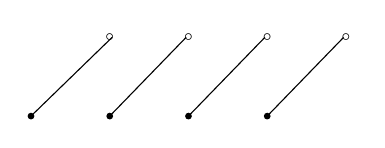
\begin{tikzpicture}
		    % abscisa y ordenada
		    \tkzInit[xmax= 2,xmin=-2,ymax=1,ymin=-1]
		    \tiny\tkzLabelXY[opacity=0.6,step=1, orig=false]
		    % label x, f(x)
		    \tkzDrawX[opacity= .6,label=x,right=0.3]
		    \tkzDrawY[opacity= .6,label=f(x),below = -0.6]
		    %funciones
		    \draw(-2,0)--(-.97,1);
		    \draw(-1,0)--(-0.03,1);
		    \draw(0,0)--(0.97,1);
		    \draw(1,0)--(1.97,1);
		    %puntos
		    \filldraw[black](-2,0) circle(1pt);
		    \draw(-1,1)node[]{$\circ$};
		    \filldraw[black](-1,0) circle(1pt);
		    \draw(0,1)node[]{$\circ$};
		    \filldraw[black](0,0) circle(1pt);
		    \draw(1,1)node[]{$\circ$};
		    \filldraw[black](1,0) circle(1pt);
		    \draw(2,1)node[]{$\circ$};
		\end{tikzpicture}
	    \end{center}
	    \vspace{.5cm}

	%----------(iii)
	\item $f(x)=\sqrt{x - [x]}$\\\\

	%----------(iv)
	\item $f(x)=[x] + \sqrt{x - [x]}$\\\\

	%----------(v)
	\item $f(x)=\left[\dfrac{1}{x}\right]$\\\\

	%----------(vi)
	\item $f(x)=\dfrac{1}{\left[\dfrac{1}{x}\right]}$\\\\

    \end{enumerate}

    %--------------------18.
    \item Trazar la gráfica de las funciones siguientes:
    \begin{enumerate}[\bfseries (a)]
	
	%----------(i)
	\item $f(x)={x},$ donde ${x}$ es la distancia de $x$ al entero más próximo\\\\
	
	%----------(ii)
	\item $f(x)={2x}$\\\\
	
	%----------(iii)
	\item $f(x)={x}+\frac{1}{2}{2x}$\\\\
	
	%----------(iv)
	\item $f(x)={4x}$\\\\
	
	%----------(v)
	\item ${x} + \frac{1}{2}{2x} + \frac{1}{4}{4x}$\\\\

    \end{enumerate}

    %--------------------19.
    \item Describir lo mejor que se pueda las gráficas de las funciones siguientes.\\\\
    \begin{enumerate}[\bfseries (i)]
	
	%----------(i)
	\item $f(x)=$ el primer número del desarrollo decimal de $x$.\\\\

	%----------(ii)
	\item $f(x)=$ el segundo número del desarrollo decimal de $x$.\\\\

	%----------(iii)
	\item $ff(x)=$ el número de sietes del desarrollo decimal de $x$ si este número es finito, y $0$ en el caso contrario.\\\\

	%----------(iv)
	\item $f(x)=0$ si el número de sietes del desarrollo decimal de $x$ es finito y $1$ en el caso contrario.\\\\

	%----------(v)
	\item $f(x)=$ el número obtenido sustituyendo todas las cifras del desarrollo decimal de $x$ que vienen después del primer $7$ si la hay por $0$.\\\\

	%----------(vi)
	\item $f(x)=0$ si $1$ no aparece en el desarrollo decimal de $x$, y $n$ si $1$ aparece por primera vez en el n-ésimo lugar.\\\\
    \end{enumerate}

    %--------------------20.
    \item Sea $$f(x)=\left\{ \begin{array}{rl}
	0,&x \; irracional\\
	\\ \frac{1}{q},& x=\frac{p}{q} \mbox{racional en forma irreducible}\\\\
    \end{array}\right.$$

    %--------------------21.
    \item
    \begin{enumerate}[\bfseries (a)]
	
	%----------(a)
	\item Los puntos de la gráfica de $f(x)=x^2$ son los de la forma $(x,x^2)$. Demostrar que cada uno de tales puntos equidista del punto $(0,\frac{1}{4})$ y de la gráfica de $g(x)=-\frac{1}{4}$.\\\\
	    Demostrar.-\; Supongamos que la distancia $d_1 = d_2$ siendo $d_1$ la distancia entre $(x,x^2)$ y $(0,\frac{1}{4})$ y $d_2$ la distancia entre $(x.x^2)$ y $(x,-\frac{1}{4})$ entonces $$(x-0)^2+\left(x^2-\frac{1}{4}\right)^2 = (x-x)^2 + \left(x^2+\frac{1}{4}\right)^2 \quad \Rightarrow \quad \left(x^2 + \frac{1}{4}\right)^2 = \left(x^2 + \frac{1}{4}\right)^2$$ por lo tanto queda demostrada la proposición.\\\\

	%----------(b)
	\item Dado un punto $P=(\alpha,\beta)$ y una recta horizontal $L,$ gráfica de la función $g(x)=\gamma$, demostrar que el conjunto de todos los puntos $(x,y)$ que equidistan de $P$ y $L$ es la gráfica de una función de la forma $f(x)=ax^2 + bx + c$.\\\\
	Demostración.-\; El punto $(x,y)$ satisface esta condición si y sólo si $$(x-\alpha)^2 + (y-\beta)^2 = (y-\gamma)^2$$ es decir $$y=\left(\dfrac{1}{2\beta - 2 \gamma}\right)x^2 + \left(\dfrac{\alpha}{\gamma - \beta}\right) x + \left(\dfrac{\alpha^2 + \beta^2 - \gamma^2}{2\beta - 2\gamma}\right)$$ siempre que $\beta \neq \gamma$.\\\\

    \end{enumerate}

    %--------------------22.
    \item 
    \begin{enumerate}[\bfseries (a)]
	
	%----------(a)
	\item Demostrar que el cuadrado de la distancia de $(c,d)$ a $(x,mx)$ es $$x^2(m^2+1)+x(-2md-2c)+d^2+c^2$$ Utilizando el problema $1-18$ para encontrar el mínimo de estos números demostrar que la distancia de $(c,d)$ a la gráfica $f(x)=mx$ es $$|cm-d|/\sqrt{m^2+1}$$\\\\
	    Demostración.-\; La demostrar de la primera parte es sencilla si tomamos $(x-c)^2+(mx-d)^2$.\\
	    Luego según $1-18$ el mínimo de dos números se encuentra mediante $c-\dfrac{b^2}{4a}$ se tiene $d^2 + c^2 - \dfrac{(-2md-2c)^2}{4(m^2+1)}$ resolviendo nos queda $\dfrac{(cm-d)^2}{m^2+1}$.\\\\

	%----------(b)
	\item Hallar la distancia de $(c,d)$ a la gráfica de $f(x)=x+b$. Reducir este caso a la parte $(a)$.\\\\
	    Respuesta.-\; La distancia de $(c,d)$ a la gráfica de $f$ es la misma que la distancia de $(c,d-b)$ a la gráfica de $g(x)=mx$. Entones por la parte $(a)$, nos queda $$\dfrac{|cm-d+b|}{m^2+1}$$.\\\\
    \end{enumerate}

    %--------------------23.
    \item 
    \begin{enumerate}[\bfseries (a)]
	
	%----------(a)
	\item Utilizando el problema $22$, demostrar que los número $x^{'}$ e $y^{'}$ indicados en la figura $31$ vienen dados por $$x^{'} = \dfrac{1}{\sqrt{2}}x + \dfrac{1}{\sqrt{2}}y,$$ $$y^{'}= - \dfrac{1}{\sqrt{2}}x + \dfrac{1}{\sqrt{2}}y$$\\\\
	    Demostración.-\; Debido a que el todos los ángulos que forman estas rectas son $45^{\circ}$ se tiene $f(x)=-x$ y $g(x)=x$ entonces por el problema anterior nos queda $$x^{'}=\dfrac{|-x-y|}{\sqrt{2}} = |-1|\cdot \left| \dfrac{x}{\sqrt{2}} + \dfrac{y}{\sqrt{2}}\right|,$$ $$y^{'} = \dfrac{|x-y|}{\sqrt{2}}= \left|\dfrac{x}{\sqrt{2}} - \dfrac{y}{\sqrt{2}}\right|$$\\\\

	%----------(b)
	\item Demostrar que el conjunto de todos los $(x,y)$ con $(x^{'} / \sqrt{2})^2 - (y^{'}/\sqrt{2})^2 = 1$ es lo mismo que el conjunto de todos los $(x,y)$ con $xy=1$.\\\\
	    Demostración.-\; Al ser $$\dfrac{x^{'}}{\sqrt{2}} = \dfrac{x}{2} + \dfrac{y}{2},$$ $$\dfrac{y^{'}}{\sqrt{2}}=-\dfrac{x}{2}+\dfrac{y}{2}$$ luego 
	    \begin{center}
		\begin{tabular}{ccl}
		    $1$&$=$&$\left( \dfrac{x}{2} + \dfrac{y}{2} \right)^2 - \left( - \dfrac{x}{2} + \dfrac{y}{2} \right)^2$\\\\
		    &$=$&$\dfrac{x^2}{4} + \dfrac{y^2}{4} + \dfrac{xy}{2} - \left( \dfrac{x^2}{4} + \dfrac{y^2}{4} - \dfrac{xy}{2} \right)$\\\\
		    &$=$&$xy$\\\\
		\end{tabular}
	    \end{center}
	    
    \end{enumerate}

\end{enumerate}

\section{Problemas}

\begin{enumerate}[\Large \bfseries 1.]

    %--------------------1.
    \item Demostrar que si dos puntos tienen por coordenadas polares $(r_1,\theta_1)$ y $(r_2,\theta_2)$, la distancia $d$ entre ellos viene dada por $$d^2 = r_1^2 + r_2^2 - 2r_1 r_2 \cos(\theta_1 - \theta_2).$$\\
	Demostración.-\; 
	\begin{center}
	    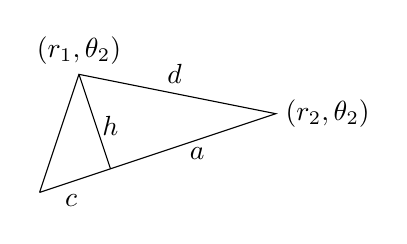
\begin{tikzpicture}
		\draw(0,0)--(3,1)node[right]{$(r_2,\theta_2)$}--(.5,1.5)node[above]{$(r_1,\theta_2)$}--(0,0);
		\draw(.5,1.5)--(.9,.3);
		\draw(1.5,1.5)node[right]{$d$};
		\draw(.9,.6)node[above]{$h$};
		\draw(.4,.1)node[below]{$c$};
		\draw(2,.7)node[below]{$a$};
	    \end{tikzpicture}
	\end{center}
	Por el teorema de Pitágoras se tiene $d^2 = a^2 + h^2$ y $r_1^2 = h^2 + c^2$ entonces $d^2 = a^2 + r_1^2 + c^2$. Luego $r_2 = c+a$ y por lo tanto $d^2 =  (r_2 - c)^2 + r_1^2 - c^2 \quad  \Rightarrow \quad d^2 = r_1^2 + r_2^2 - 2r_2c$. Nótese que $c=r_1\cos(\theta_1-\theta_2)$ y por lo tanto $$d^2 = r_1^2 + r_2^2 - 2r_1 r_2 \cos(\theta_1 - \theta_2)$$\\

\end{enumerate}
